\documentclass{standalone}
\usepackage{pgfplots}
\usepackage{amsmath}
\usepgfplotslibrary{colormaps}
\usetikzlibrary{math}

\pgfplotsset{compat=newest}
%%%% Differential system %%%%%
%\def\c{1}
\def\a{2}
\def\b{1.5}
\def\xdot{x*(1-x-\a*y)}
\def\ydot{y*(1-y-\b*x)}
%%%%%%%%%%%%%%%%%%%%%%%%%%%%%%

\begin{document}
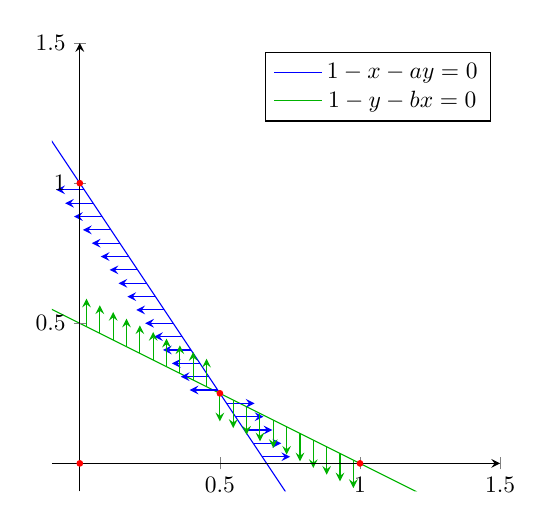
\begin{tikzpicture}[every node/.style={scale=0.85}]
  \begin{axis}[
      axis lines=middle,
      xmin=-0.1,xmax=1.5,
      ymin=-0.1, ymax=1.5,
      zmin = 0, zmax = 1, % to prevent a warning
      view={0}{90},
      % xlabel = {$x$},
      % ylabel = {$y$},
      axis equal image,
      trig format plots=rad,
      %colormap/vidris,
      %axis on top=false,
    ]
    \def\xmax{\pgfkeysvalueof{/pgfplots/xmax}}
    \def\xmin{\pgfkeysvalueof{/pgfplots/xmin}}
    \def\ymax{\pgfkeysvalueof{/pgfplots/ymax}}
    \def\ymin{\pgfkeysvalueof{/pgfplots/ymin}}
    % \addplot3[
    % opacity = 0.5,
    % point meta={sqrt((\xdot)^2+(\ydot)^2)},
    % samples=17,
    % domain=\xmin:\xmax,
    % y domain=\xmin:\xmax,
    % quiver={
    % u={\xdot/sqrt((\xdot)^2+(\ydot)^2)},
    % v={\ydot/sqrt((\xdot)^2+(\ydot)^2)},
    % colored = {mapped color},
    % scale arrows=0.05,
    % every arrow/.append style={-{stealth}}
    % }
    % ] {0};
    % \foreach \i in{(\b-1)/(\a-1)*x}{
    %     \addplot[
    %       samples=200,
    %       % samples y=100,
    %       domain=\xmin:\xmax,
    %       %y domain=\xmin:\xmax,
    %       red
    %     ] {\i};
    %   }
    \addplot[blue]{1-\b*x};
    \addplot[green!70!black]{(1-x)/\a};
    % \pgfmathsetmacro\px{(\a-1)/(\a*\b-1)}
    \tikzmath{
      \px=(\a-1)/(\a*\b-1);
      \py=(\b-1)/(\a*\b-1);
    }
    \def\n{20}
    \def\len{0.1}
    \makeatletter
    \newcommand{\compareb}[2]{%
    \ifdim\dimexpr#1pt<#2pt
      \edef\x {\noexpand \draw[-{stealth},blue] (\x,\y) -- ({\x-\len},\y)}%
      \x;
    \else
      \edef\x {\noexpand \draw[-{stealth},blue] (\x,\y) -- ({\x+\len},\y)}%
      \x;
    \fi
    }
    \newcommand{\compareg}[2]{%
    \ifdim\dimexpr#1pt<#2pt
      \edef\x {\noexpand \draw[-{stealth},green!70!black] (\x,\y) -- (\x,{\y+\len})}%
      \x;
    \else
      \edef\x {\noexpand \draw[-{stealth},green!70!black] (\x,\y) -- (\x,{\y-\len})}%
      \x;
    \fi
    }
    \makeatother
    % blue
    \foreach \i[evaluate={\x={(\i+0.5)/(\n+1)*1/\b};\y={1-\b*\x}}] in {0,...,\n}
      {%
        \compareb{\x}{\px}
      }
    % green
    \foreach \i[evaluate={\y={(\i+0.5)/((\n+1)*\a)};\x={1-\a*\y}}] in {0,...,\n}
      {%
        \compareg{\x}{\px}
      }
    \addplot[thin,mark=*,only marks, mark size=1pt,red] coordinates {
        (0,0) (1,0) (0,1) ({(\a-1)/(\a*\b-1)},{(\b-1)/(\a*\b-1)})
      };
    \legend{$1-x-ay=0$,$1-y-bx=0$}
  \end{axis}
\end{tikzpicture}
\end{document}